\documentclass{article}
\usepackage{german}
\usepackage{a4, fullpage, times, graphicx, rotating}
\usepackage{isolatin1}
\usepackage[screen,buttons]{powerslide}
\usepackage{pause}
\usepackage{default}
\title{LINBO}
\author{Klaus Knopper $<$knopper@knopper.net$>$\\
Martin �hler $<$oehler@knopper.net$>$}
\date{Stand: 25.9.2007\\[3mm]
\colorbox{white}{
\includegraphics[width=0.5\textwidth]{pics/png/linbo-logo.png}}}
\hypersetup{pdfpagetransition=Dissolve}
\def\myurl#1{\href{#1}{\textbf{\texttt{#1}}}}
\renewcommand{\labelitemi}{\ding{237}}
\renewcommand{\labelitemii}{\ding{235}}
\renewcommand{\rightarrow}{\ding{43}}%
\def\X{\ding{52}}


% Lighter colors for screen version
\definecolor{lightyellow}{rgb}{1,1,.9}
\definecolor{red}{rgb}{1,.4,.4}
\definecolor{green}{rgb}{.4,1,.4}
\definecolor{blue}{rgb}{.4,.4,1}
\definecolor{yellow}{cmyk}{0,0,.6,0}
\definecolor{cyan}{cmyk}{.6,0,0,0}
\definecolor{magenta}{cmyk}{0,.6,0,0}

\def\kdo#1{\textbf{\texttt{#1}}}

%\newsavebox{\logo}
%\sbox{\logo}{\setlength{\unitlength}{1mm}
%\begin{picture}(40,5)
%\put(0,0){\includegraphics[width=4cm]{pics/logo/iirlogo.pdf}}
%\end{picture}}
\newsavebox{\mycopyright}
\sbox{\mycopyright}{{\footnotesize\raise0.2ex\hbox{$\copyright$} 2007 Klaus Knopper}}
\newsavebox{\knopper}
\sbox{\knopper}{{\footnotesize $<$knopper@knopper.net$>$}}
%\rhead{\usebox{\logo}}
% \lhead{\thesection}
% \rfoot{{\footnotesize{}Folie \thepage~von~\pageref{lastpage}}}
\fontfamily{phv}\selectfont
\renewcommand{\rmdefault}{phv}
\begin{document}
\slidemaketitle
% \setbgcolor{blue1}
\begin{slidepage}{Zusammenfassung}
\colorbox{black}{%
\begin{fancybox}
\vspace*{2mm}

%\begin{small}
\color{black}
\begin{itemize}
\item Open Source Boot- und Installationsmanager,
\item OS-unabh�ngige Installation, Reparatur, Synchronisation,
\item Startet lokal (MBR, ISO, Flash) und Remote (PXE),
\item Special Features:
\begin{itemize}
\item Cache-Initialisierung per Multicast (optional),
\item NTFS-Schreibsupport mit ntfs-3g \rightarrow\ Vista$^{\mbox{\tiny TM}}$-Ready,
\item Integrierter, automatischer Registry-Patcher,
\item Erweiterbare graphische Oberfl�che (embedded QT),
\item Integriert in PaedML$^{\mbox{\tiny TM}}$.
\end{itemize}
\end{itemize}
%\end{small}
\end{fancybox}}
\end{slidepage}

\begin{slidepage}{LINBO - Kernteile}

\begin{itemize}
\item LINBO-OS (GNU/Linux Mini System, KNOPPIX-�hnlich),
\item ~~Frontend / Graphische Oberfl�che \kdo{linbo\_gui},
\item ~~Backend / Shellskript \kdo{linbo\_cmd},
\item ~~Busybox (Shell) und Utilities, auch f�r Experten.
\end{itemize}

\end{slidepage}

\begin{slidepage}{LINBO - OS}

\begin{itemize}
\item Linux-Kernel (aktuelle Version: 2.6.21.7)
\item Initramfs mit LINBO-Kernteilen sowie
\item cloop 2.06 (\rightarrow\ 2.622)
\end{itemize}

\rightarrow\ 2 Bootdateien gen�gen zur Installation,\\
\rightarrow\ Lokal (lilo, isolinux) wie remote (PXE) bootbar.

\end{slidepage}

\begin{slidepage}{LINBO - Server-Seite}
\begin{itemize}
\item DHCPD, TFTPS (f�r PXE-Boot),
\item RSYNC-Server,
\item LINBO-OS und Images,
\item Webgui oder Editor zur Konfiguration (start.conf).
\end{itemize}
\end{slidepage}

\begin{slidepage}{LINBO - Installation}

Manuell: 2 Dateien (\kdo{linbo} und \kdo{linbofs.gz}) an die
richtigen Stellen im DHCP/TFTP-Bootserver kopieren und eintragen, oder

\bigskip

Debian-Paket: \kdo{dpkg -i linuxmuster-linbo\_1.0-1\_i386.deb}

\bigskip

F�r die administrativen Funktionen (Anmeldung, Images hochladen) muss
der RSYNC-Server entsprechend konfiguriert werden.
\end{slidepage}

\begin{slidepage}{LINBO - RSYNC}
RSYNC unterst�tzt effizientes �bertragen und Updaten von Bin�rdateien, sowie
ein sicheres Authentifikations- und Rechtesystem.

Beispiel:
\kdo{/etc/rsyncd.conf}

\begin{center}
\begin{tabular}{l|l}
\begin{minipage}[t]{5cm}
\begin{verbatim}
[linbo]
 comment = LINBO Images
 path = /var/linbo
 read only = yes
 list = yes
\end{verbatim}
\end{minipage} &
\begin{minipage}[t]{5cm}
\begin{verbatim}
[linbo-upload]
 comment = LINBO Uploads
 path = /var/linbo
 read only = no
 auth users = linbo
 secrets file = \
     /etc/rsyncd.secrets
\end{verbatim}
\end{minipage}
\end{tabular}
\end{center}
\end{slidepage}

\begin{slidepage}{LINBO - \kdo{start.conf} Konfiguration (1)}
Globale Einstellungen (pro Rechner/Gruppe):
\begin{verbatim}
[LINBO]
Cache = /dev/hda6       # Cache Partition
Server = 10.0.2.2       # RSYNC-Server mit Images
RootTimeout = 180       # Timeout f�r Admin
\end{verbatim}
\end{slidepage}

\begin{slidepage}{LINBO - \kdo{start.conf} Konfiguration (2)}
Partitionen:
\begin{verbatim}
[Partition]
Dev = /dev/hda1         # Linux Device Name
Size = 4200997          # Partitionsgr��e in kB
Id = 7                  # Partitions Typ (7 = NTFS)
FSType = ntfs           # Dateisystem
Bootable = yes          # "Bootbar" Kennzeichnung
\end{verbatim}
\end{slidepage}

\begin{slidepage}{LINBO - \kdo{start.conf} Konfiguration (3)}
Betriebssysteme (Windows):
\begin{verbatim}
[OS]
Name = Windows Visa SP 666 
Description = 06.02.2007, 10:10 Es bootet.
Version = 1.0
Image = xp-20070727.rsync
BaseImage  = xp.cloop
Boot = /dev/hda1
Root = /dev/hda1
Kernel = grub.exe # Secondary Bootlader
Initrd = 
Append = --config-file=map(rd)+1 (hd0,0); \
         map --hook; chainloader (hd0,0)+1; \
         rootnoverify(hd0,0) --device-map=(hd0) \
         /dev/hda          # grub-Konfiguration
StartEnabled = yes # "Start" Button zeigen
\end{verbatim}
\end{slidepage}

\begin{slidepage}{LINBO - \kdo{start.conf} Konfiguration (4)}
Betriebssysteme (Linux):
\begin{verbatim}
[OS]
Name = Mini-Knoppix
Version = 5.2
Description = 01.02.2007, 7:10 HD-Install
Image =         # Kein diff. Image n�tig.
BaseImage  = microknoppix.cloop
Boot = /dev/hda5
Root = /dev/hda5
Kernel = vmlinuz
Initrd = initrd.gz
Append = acpi=off quiet
\end{verbatim}
\end{slidepage}


\begin{slidepage}{Imaging mit LINBO - Funktionsweise}
\begin{center}
\colorbox{white}{\textcolor{black}{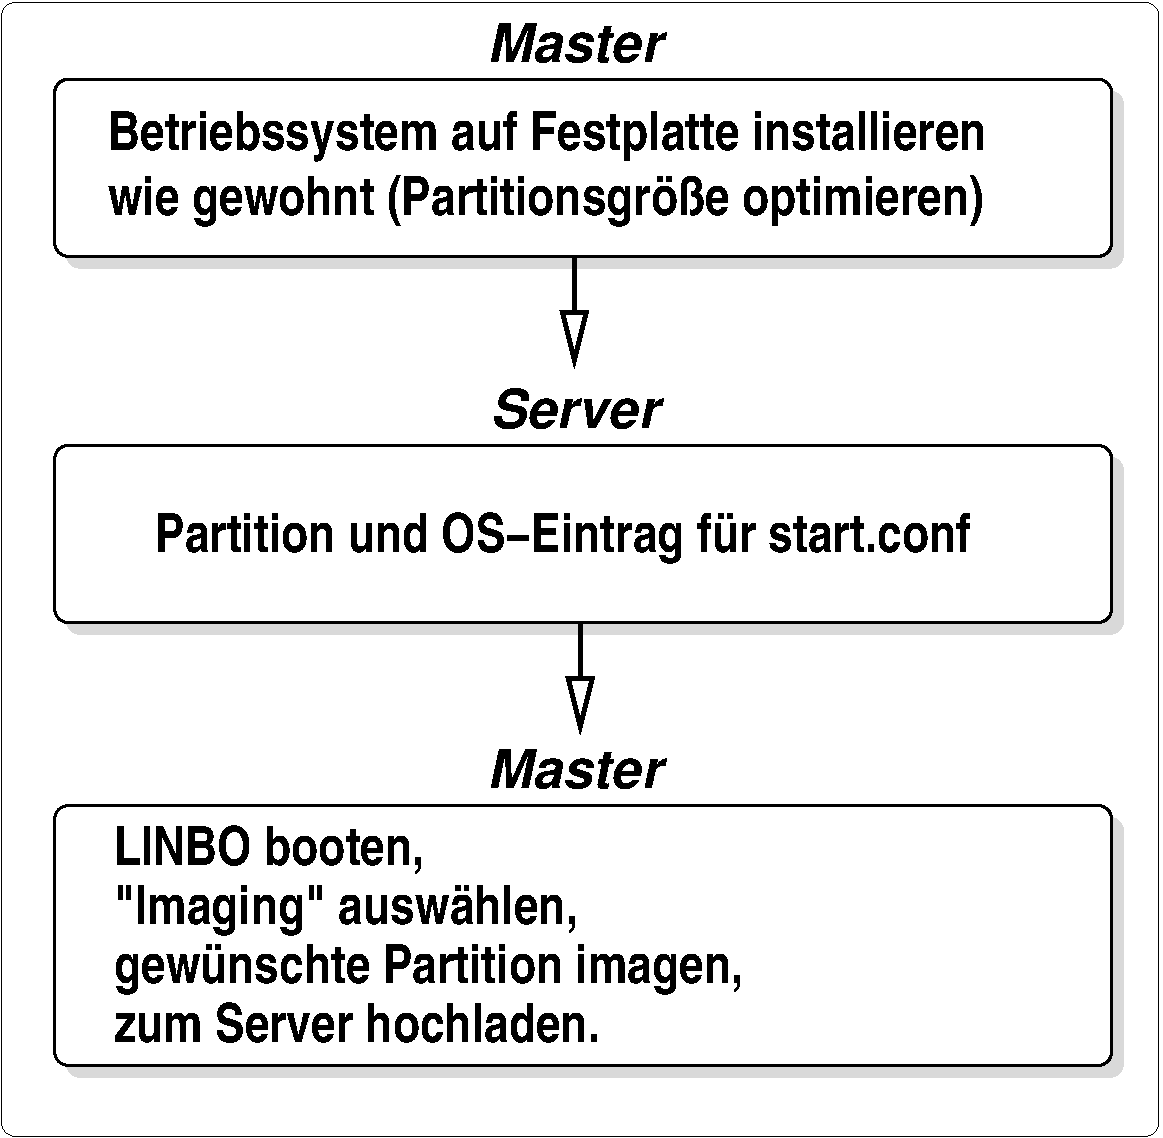
\includegraphics[width=0.5\textwidth]{pics/pdf/imaging-funktionsweise.pdf}}}
\end{center}
\end{slidepage}

\begin{slidepage}{Image - Typen}

Jedes von LINBO verwaltete Betriebssystem besteht aus einem \textsl{Basis-Image}, plus h�chstens einem \textsl{Differentiellen Image}.

\begin{description}
\item [\kdo{.cloop}:] Kompletter, cloop-komprimierter Partitionsdump (1:1 Kopie), dateisystemunabh�ngig. Wird f�r \textsl{Basis-Images} verwendet.
\item [\kdo{.rsync}:] "`rsync-Batch"', komprimiertes, rsync-eigenes Datenformat, wird f�r \textsl{Differentielle Images} verwendet.
\end{description}

% \kdo{.reg}: Registry-Patches (nur bei Windows erforderlich).

\begin{center}
\colorbox{white}{\textcolor{black}{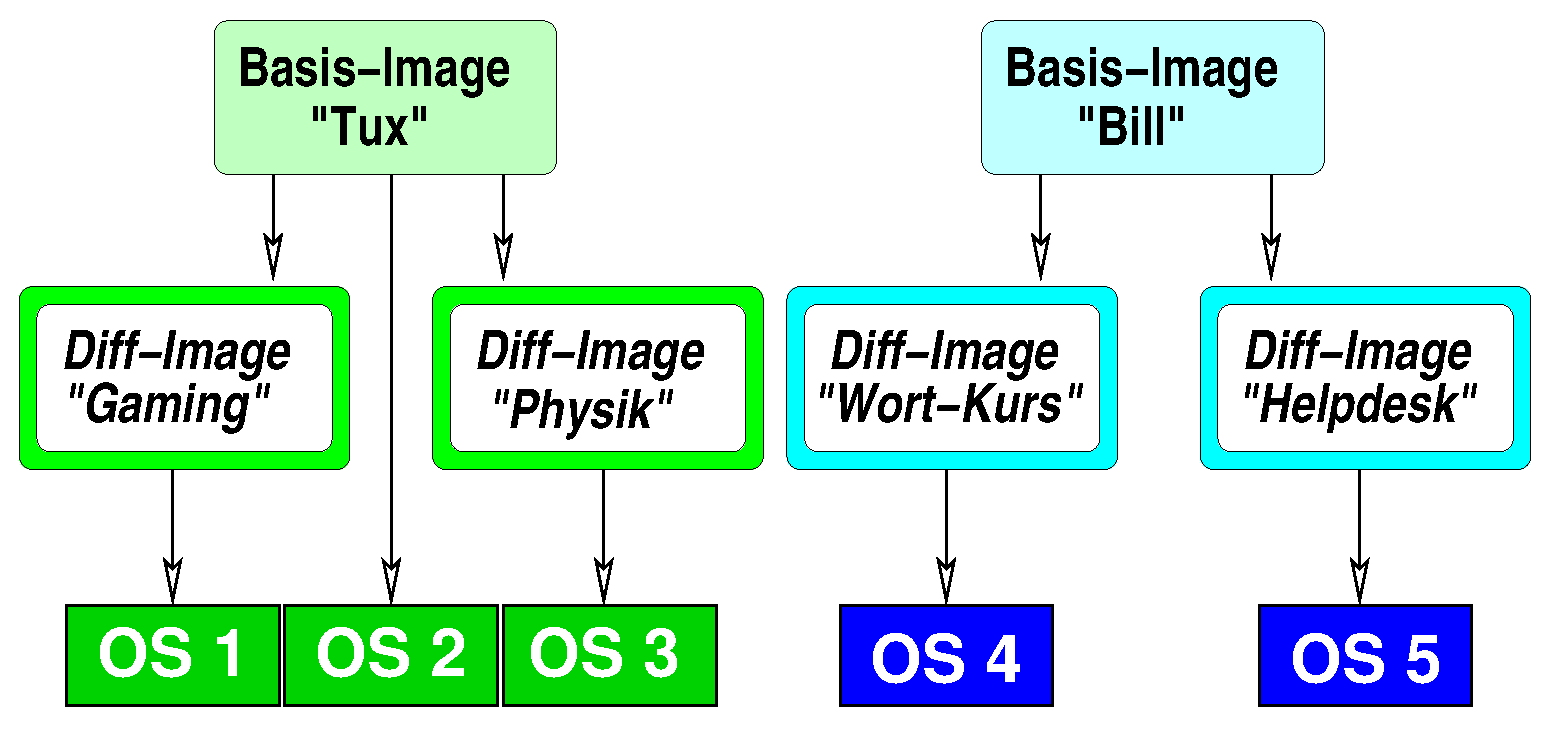
\includegraphics[height=0.15\textheight]{pics/pdf/image-typen.pdf}}}
\end{center}

\end{slidepage}

\begin{slidepage}{LINBO - GUI}

\vspace*{\fill}

\begin{center}
\LARGE
...Bitte umbl�ttern (live)...
\end{center}

\vspace*{\fill}

\end{slidepage}

\begin{slidepage}{Cache aufladen - Multicast}

Um eine Anzahl von Rechnern \underbar{gleichzeitig} mit Images zu versorgen, bietet sich Muticast an (implementiert durch \kdo{udpcast}):

Vorteile:

\begin{itemize}
\item Jedes Image muss nur einmal �bertragen werden,
\item Mehrere Rechner empfangen das gleiche Image zur selben Zeit,
\item Falls \kdo{udp-server} nicht zur Verf�gung steht (z.B. bei Windows-Rechner als Server), kann auf \kdo{rsync} zur�ckgegriffen werden.
\end{itemize}
\end{slidepage}

\begin{slidepage}{LINBO - Status}

\begin{center}
\begin{tabular}{|l|c|c|c|c|}\hline
Feature & ~~\begin{sideways}Produktiv\end{sideways}~~ & ~~\begin{sideways}Testphase\end{sideways}~~ & ~~\begin{sideways}In Entwicklung\end{sideways}~~ & ~~\begin{sideways}Wunschliste\end{sideways}~~~\\\hline\hline
Installation & \X{} & & &  \\\hline
Wiederherstellung & \X{} & & & \\\hline
Imaging & \X{} & & & \\\hline
OS: Linux & \X{} & & & \\\hline
OS: Win 98 & & \X{} & & \\\hline
OS: Win XP & & \X{} & & \\\hline
Windows-Patches & & \X{} & & \\\hline
OS: Win Vista & & & \X{} & \\\hline
Webgui & & & \X{} & \\\hline
Mac-Version & & & & \X{} \\\hline
\end{tabular}
\end{center}

\end{slidepage}
\end{document}
